% questions.tex —— 2010 年·普通高等学校招生考试·浙江卷·理科 · 题目内容片段（无答案）
% 由 tools/generate_projects.py 依来源总账自 2010/2010_数学真题_浙江理_试题.md 生成，勿手改（改源 MD 后重跑）
状态：needs-review；依固定候选 PDF 两页（印刷页 639–640）逐题核验，五幅图已矢量重绘。原页未印分值，不补。
\gkpart{一、选择题}
\begin{question}
\gkti{1}设 $P=\{x\mid x<4\}$，$Q=\{x\mid x^2<4\}$，则（　）

（A）$P\subseteq Q$

（B）$Q\subseteq P$

（C）$P\subseteq\complement_{\mathbf R}Q$

（D）$Q\subseteq\complement_{\mathbf R}P$

\Needspace{0.4\textheight}
\end{question}
\begingroup
\renewenvironment{question}{\Needspace{0.5\textheight}}{}
\begin{question}
\gkti{2}某程序框图如图所示，若输出的 $S=57$，则判断框内为（　）

（A）$k>4$?

（B）$k>5$?

（C）$k>6$?

（D）$k>7$?
\nopagebreak[4]
\begin{center}% 2010 年浙江卷理科第 2 题：程序框图（判断框内容待填）。
% 来源 PDF：普通高考/2010/2010浙江理.pdf，SHA-256 c61b26c8cab009d567644272afc34d81e3174ffa90244c333ecfb27d61034a00。
% 原页：第 1 页（A3 三栏）第 1 栏上部，书页码 639。
% 重绘依据：照原页流程，开始→S=1,k=1→k=k+1→S=2S+k→判断框；
%   判断框“是”向下经“输出 S”到“结束”，“否”自左侧折回 k=k+1 上方。
\begin{tikzpicture}[scale=1.0, semithick,
  every node/.style={inner sep=2pt},
  box/.style={draw, minimum width=2.4cm, minimum height=0.58cm, align=center},
  round/.style={draw, rounded corners=5pt, minimum width=1.4cm,
    minimum height=0.58cm, align=center},
  para/.style={draw, trapezium, trapezium left angle=70, trapezium right angle=110,
    minimum width=2.2cm, minimum height=0.6cm, align=center},
  dec/.style={draw, diamond, aspect=2.2, minimum width=3.0cm,
    minimum height=1.15cm, align=center},
  arr/.style={->, >=stealth}]

  \node[round] (start) at (0,8.4) {开始};
  \node[box]   (init)  at (0,7.35) {$S=1,\ k=1$};
  \node[box]   (inc)   at (0,5.75) {$k=k+1$};
  \node[box]   (sum)   at (0,4.55) {$S=2S+k$};
  \node[dec]   (test)  at (0,3.05) {};
  \node[para]  (out)   at (0,1.75) {输出 $S$};
  \node[round] (end)   at (0,0.7)  {结束};

  \draw[arr] (start) -- (init);
  \draw[arr] (init) -- (inc);
  \draw[arr] (inc) -- (sum);
  \draw[arr] (sum) -- (test);
  \draw[arr] (test.south) -- (out.north);
  \node[right] at (0.12,2.35) {是};
  \draw[arr] (out) -- (end);
  \draw[arr] (test.west) -- (-2.35,3.05) -- (-2.35,6.55) -- (0,6.55);
  \node[left] at (-2.35,4.45) {否};
\end{tikzpicture}
\end{center}
\nopagebreak[4]
\end{question}
\endgroup
\begin{question}
\gkti{3}设 $S_n$ 为等比数列 $\{a_n\}$ 的前 $n$ 项和，$8a_2+a_5=0$，则 $\dfrac{S_5}{S_2}=$（　）

（A）$11$

（B）$5$

（C）$-8$

（D）$-11$

\end{question}
\begin{question}
\gkti{4}设 $0<x<\dfrac{\pi}{2}$，则“$x\sin^2x<1$”是“$x\sin x<1$”的（　）

（A）充分而不必要条件

（B）必要而不充分条件

（C）充分必要条件

（D）既不充分也不必要条件

\end{question}
\begin{question}
\gkti{5}对任意复数 $z=x+y\mathrm i$（$x,y\in\mathbf R$），$\mathrm i$ 为虚数单位，则下列结论正确的是（　）

（A）$|z-\bar z|=2y$

（B）$z^2=x^2+y^2$

（C）$|z-\bar z|\geqslant 2x$

（D）$|z|\leqslant |x|+|y|$

\end{question}
\begin{question}
\gkti{6}设 $l$，$m$ 是两条不同的直线，$\alpha$ 是一个平面，则下列命题正确的是（　）

（A）若 $l\perp m$，$m\subset\alpha$，则 $l\perp\alpha$

（B）若 $l\perp\alpha$，$l\parallel m$，则 $m\perp\alpha$

（C）若 $l\parallel\alpha$，$m\subset\alpha$，则 $l\parallel m$

（D）若 $l\parallel\alpha$，$m\parallel\alpha$，则 $l\parallel m$

\end{question}
\begin{question}
\gkti{7}若实数 $x$，$y$ 满足不等式组
\nopagebreak[4]
\[\begin{cases}
x+3y-3\geqslant 0,\\
2x-y-3\leqslant 0,\\
x-my+1\geqslant 0,
\end{cases}\]
且 $x+y$ 的最大值为 $9$，则实数 $m=$（　）

（A）$-2$

（B）$-1$

（C）$1$

（D）$2$

\end{question}
\begin{question}
\gkti{8}设 $F_1$、$F_2$ 分别为双曲线 $\dfrac{x^2}{a^2}-\dfrac{y^2}{b^2}=1$（$a>0$，$b>0$）的左、右焦点。若在双曲线右支上存在点 $P$，满足 $|PF_2|=|F_1F_2|$，且 $F_2$ 到直线 $PF_1$ 的距离等于双曲线的实轴长，则该双曲线的渐近线方程为（　）

（A）$3x\pm 4y=0$

（B）$3x\pm 5y=0$

（C）$4x\pm 3y=0$

（D）$5x\pm 4y=0$

\end{question}
\begin{question}
\gkti{9}设函数 $f(x)=4\sin(2x+1)-x$，则在下列区间中函数 $f(x)$ 不存在零点的是（　）

（A）$[-4,-2]$

（B）$[-2,0]$

（C）$[0,2]$

（D）$[2,4]$

\end{question}
\begin{question}
\gkti{10}设函数的集合
\nopagebreak[4]
\[P=\left\{f(x)=\log_2(x+a)+b\ \middle|\ a=-\frac12,0,\frac12,1;\ b=-1,0,1\right\},\]
\Needspace{5\baselineskip}
平面上点的集合
\nopagebreak[4]
\[Q=\left\{(x,y)\ \middle|\ x=-\frac12,0,\frac12,1;\ y=-1,0,1\right\},\]
则在同一直角坐标系中，$P$ 中函数 $f(x)$ 的图象恰好经过 $Q$ 中两个点的函数的个数是（　）

（A）$4$

（B）$6$

（C）$8$

（D）$10$

\end{question}
\gkpart{二、填空题}
\begin{question}
\gkti{11}函数 $f(x)=\sin\left(2x-\dfrac{\pi}{4}\right)-2\sqrt2\sin^2x$ 的最小正周期是 $\underline{\qquad}$。

\Needspace{0.4\textheight}
\end{question}
\begingroup
\renewenvironment{question}{\Needspace{0.5\textheight}}{}
\begin{question}
\gkti{12}若某几何体的三视图（单位：cm）如图所示，则此几何体的体积是 $\underline{\qquad}$ cm$^3$。
\nopagebreak[4]
\begin{center}% 2010 年浙江卷理科第 12 题：三视图（正视图、侧视图、俯视图）。
% 来源 PDF：普通高考/2010/2010浙江理.pdf，SHA-256 c61b26c8cab009d567644272afc34d81e3174ffa90244c333ecfb27d61034a00。
% 原页：第 1 页（A3 三栏）第 2 栏中部，书页码 639。
% 重绘依据：正视图与侧视图均为下底 8、上底 4、高 3 的等腰梯形，其上叠 4×2 的矩形；
%   俯视图为外方 8×8、内方 4×4、四角以对角线相连。尺寸 2、4、2 与 2、3 照原页标注。
\begin{tikzpicture}[scale=0.4, semithick, every node/.style={inner sep=1.5pt, font=\small},
  dim/.style={<->, >=stealth, thin}]

  % ---------- 正视图 ----------
  \draw (-4,0) -- (4,0) -- (2,3) -- (-2,3) -- cycle;
  \draw (-2,3) rectangle (2,5);
  % 顶部尺寸 2,4,2
  \draw[thin] (-4,5.25) -- (-4,5.85);
  \draw[thin] (-2,5.25) -- (-2,5.85);
  \draw[thin] (2,5.25) -- (2,5.85);
  \draw[thin] (4,5.25) -- (4,5.85);
  \draw[dim] (-4,5.55) -- (-2,5.55);
  \draw[dim] (-2,5.55) -- (2,5.55);
  \draw[dim] (2,5.55) -- (4,5.55);
  \node[above] at (-3,5.55) {$2$};
  \node[above] at (0,5.55) {$4$};
  \node[above] at (3,5.55) {$2$};
  % 右侧尺寸 2,3
  \draw[thin] (4.15,5) -- (4.75,5);
  \draw[thin] (4.15,3) -- (4.75,3);
  \draw[thin] (4.15,0) -- (4.75,0);
  \draw[dim] (4.45,3) -- (4.45,5);
  \draw[dim] (4.45,0) -- (4.45,3);
  \node[right] at (4.45,4) {$2$};
  \node[right] at (4.45,1.5) {$3$};
  \node[below] at (0,-0.9) {正视图};

  % ---------- 侧视图 ----------
  \begin{scope}[shift={(11,0)}]
    \draw (-4,0) -- (4,0) -- (2,3) -- (-2,3) -- cycle;
    \draw (-2,3) rectangle (2,5);
    \node[below] at (0,-0.9) {侧视图};
  \end{scope}

  % ---------- 俯视图 ----------
  \begin{scope}[shift={(0,-9)}]
    \draw (-4,0) rectangle (4,-8);
    \draw (-2,-2) rectangle (2,-6);
    \draw (-4,0) -- (-2,-2);
    \draw (4,0) -- (2,-2);
    \draw (4,-8) -- (2,-6);
    \draw (-4,-8) -- (-2,-6);
    % 右侧尺寸 2,4,2
    \draw[thin] (4.15,0) -- (4.75,0);
    \draw[thin] (4.15,-2) -- (4.75,-2);
    \draw[thin] (4.15,-6) -- (4.75,-6);
    \draw[thin] (4.15,-8) -- (4.75,-8);
    \draw[dim] (4.45,-2) -- (4.45,0);
    \draw[dim] (4.45,-6) -- (4.45,-2);
    \draw[dim] (4.45,-8) -- (4.45,-6);
    \node[right] at (4.45,-1) {$2$};
    \node[right] at (4.45,-4) {$4$};
    \node[right] at (4.45,-7) {$2$};
    \node[below] at (0,-8.9) {俯视图};
  \end{scope}
\end{tikzpicture}
\end{center}
\nopagebreak[4]
\end{question}
\endgroup
\begin{question}
\gkti{13}设抛物线 $y^2=2px$（$p>0$）的焦点为 $F$，点 $A(0,2)$。若线段 $FA$ 的中点 $B$ 在抛物线上，则 $B$ 到该抛物线准线的距离为 $\underline{\qquad}$。

\end{question}
\begin{question}
\gkti{14}设 $n\geqslant 2$，$n\in\mathbf N$，
\nopagebreak[4]
\[\left(2x+\frac12\right)^n-\left(3x+\frac13\right)^n=a_0+a_1x+a_2x^2+\cdots+a_nx^n,\]
将 $|a_k|$（$0\leqslant k\leqslant n$）的最小值记为 $T_n$，则 $T_2=0$，$T_3=\dfrac1{2^3}-\dfrac1{3^3}$，$T_4=0$，$T_5=\dfrac1{2^5}-\dfrac1{3^5}$，$\cdots$，$T_n$，$\cdots$，其中 $T_n=\underline{\qquad}$。

\end{question}
\begin{question}
\gkti{15}设 $a_1$，$d$ 为实数，首项为 $a_1$，公差为 $d$ 的等差数列 $\{a_n\}$ 的前 $n$ 项和为 $S_n$，满足 $S_5S_6+15=0$，则 $d$ 的取值范围是 $\underline{\qquad}$。

\end{question}
\begin{question}
\gkti{16}已知平面向量 $\boldsymbol\alpha$，$\boldsymbol\beta$（$\boldsymbol\alpha\neq\mathbf 0$，$\boldsymbol\alpha\neq\boldsymbol\beta$）满足 $|\boldsymbol\beta|=1$，且 $\boldsymbol\alpha$ 与 $\boldsymbol\beta-\boldsymbol\alpha$ 的夹角为 $120^\circ$，则 $|\boldsymbol\alpha|$ 的取值范围是 $\underline{\qquad}$。

\end{question}
\begin{question}
\gkti{17}有 $4$ 位同学在同一天的上、下午参加“身高与体重”、“立定跳远”、“肺活量”、“握力”、“台阶”五个项目的测试，每位同学上、下午各测试一个项目，且不重复，若上午不测“握力”项目，下午不测“台阶”，其余项目上、下午都各测试一人，则不同的安排方式共有种 $\underline{\qquad}$。（用数字作答）

\end{question}
\gkpart{三、解答题}
\begin{question}
\gkti{18}在 $\triangle ABC$ 中，角 $A$、$B$、$C$ 所对的边分别为 $a$、$b$、$c$，已知 $\cos2C=-\dfrac14$。

（1）求 $\sin C$ 的值；

（2）当 $a=2$，$2\sin A=\sin C$ 时，求 $b$ 及 $c$ 的长。

\Needspace{0.4\textheight}
\end{question}
\begingroup
\renewenvironment{question}{\Needspace{0.5\textheight}}{}
\begin{question}
\gkti{19}如图，一个小球从 $M$ 处投入，通过管道自上而下落到 $A$ 或 $B$ 或 $C$。已知小球从每个叉口落入左右两个管道的可能性是相等的。某商家按上述投球方式进行促销活动，若投入的小球落到 $A$、$B$、$C$，则分别设为 $1$、$2$、$3$ 等奖。

（1）已知获得 $1$，$2$，$3$ 等奖的折扣率分别为 $50\%$、$70\%$、$90\%$。记随机变量 $\xi$ 为获得 $k$（$k=1,2,3$）等奖的折扣率，求随机变量 $\xi$ 的分布列及期望 $E\xi$；

（2）若有 $3$ 人次（投入 $1$ 球为 $1$ 人次）参加促销活动，记随机变量 $\eta$ 为获得 $1$ 等奖或 $2$ 等奖的人次，求 $P(\eta=2)$。
\nopagebreak[4]
\begin{center}% 2010 年浙江卷理科第 19 题：投球管道。
% 来源 PDF：普通高考/2010/2010浙江理.pdf，SHA-256 c61b26c8cab009d567644272afc34d81e3174ffa90244c333ecfb27d61034a00。
% 原页：第 1 页（A3 三栏）第 3 栏下部，书页码 639。
% 重绘依据：M 下第一叉口分左右；左支再分叉，左外支直达 C，内支入中；右支同理，
%   右外支直达 B，内支入中；两内支在中部汇合后再平分，左入 C、右入 A。
%   出口自左至右为 C、A、B；管道以双线表示，与原页拓扑一致。
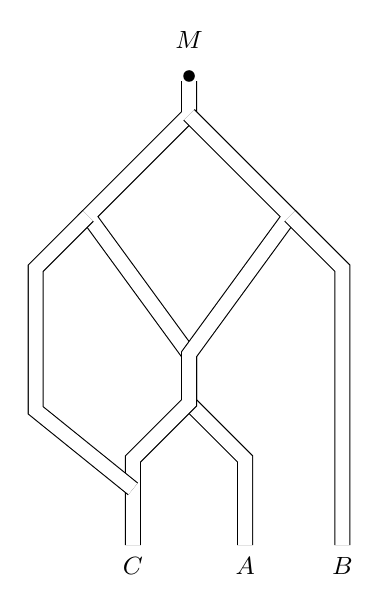
\begin{tikzpicture}[scale=0.95, every node/.style={inner sep=1.5pt, font=\small},
  pipe/.style={double, double distance=5pt, line width=0.4pt}]

  % M 至第一叉口，及左内支→中部→右叉口→A 的连续通道
  \draw[pipe] (0,7.35) -- (0,6.9) -- (-1.35,5.55) -- (0,3.7) -- (0,3.05)
    -- (0.75,2.3) -- (0.75,1.15);
  % 右内支→中部→左叉口→C 的连续通道
  \draw[pipe] (0,6.9) -- (1.35,5.55) -- (0,3.7) -- (0,3.05)
    -- (-0.75,2.3) -- (-0.75,1.15);
  % 左外支到 C
  \draw[pipe] (-1.35,5.55) -- (-2.05,4.85) -- (-2.05,2.95) -- (-0.75,1.9);
  % 右外支到 B
  \draw[pipe] (1.35,5.55) -- (2.05,4.85) -- (2.05,1.15);

  \node[below] at (-0.75,1.05) {$C$};
  \node[below] at (0.75,1.05) {$A$};
  \node[below] at (2.05,1.05) {$B$};

  % 投球点 M
  \fill (0,7.42) circle (2.2pt);
  \node[above] at (0,7.72) {$M$};
\end{tikzpicture}
\end{center}
\nopagebreak[4]
\Needspace{0.4\textheight}
\end{question}
\endgroup
\begingroup
\renewenvironment{question}{\Needspace{0.5\textheight}}{}
\begin{question}
\gkti{20}如图，在矩形 $ABCD$ 中，点 $E$，$F$ 分别在线段 $AB$、$AD$ 上，$AE=EB=AF=\dfrac23FD=4$。沿直线 $EF$ 将 $\triangle AEF$ 翻折成 $\triangle A'EF$，使平面 $A'EF\perp$ 平面 $BEF$。

（1）求二面角 $A'-FD-C$ 的余弦值；

（2）点 $M$，$N$ 分别在线段 $FD$、$BC$ 上，若沿直线 $MN$ 将四边形 $MNCD$ 向上翻折，使 $C$ 与 $A'$ 重合，求线段 $FM$ 的长。
\nopagebreak[4]
\begin{center}% 2010 年浙江卷理科第 20 题：矩形 ABCD 沿 EF 翻折为 A'EF。
% 来源 PDF：普通高考/2010/2010浙江理.pdf，SHA-256 c61b26c8cab009d567644272afc34d81e3174ffa90244c333ecfb27d61034a00。
% 原页：第 2 页（A3 三栏）第 1 栏，书页码 640。
% 重绘依据：照原页透视，D 左下、C 右下、B 右上、A 左上（原位置），E 在 AB 上，
%   F 在 AD 上；A' 在平面 BEF 上方，A'E、A'F、EF 为实线，AE、AF 为虚线；
%   M 在 FD 上、N 在 BC 上，MN 为第二折痕。
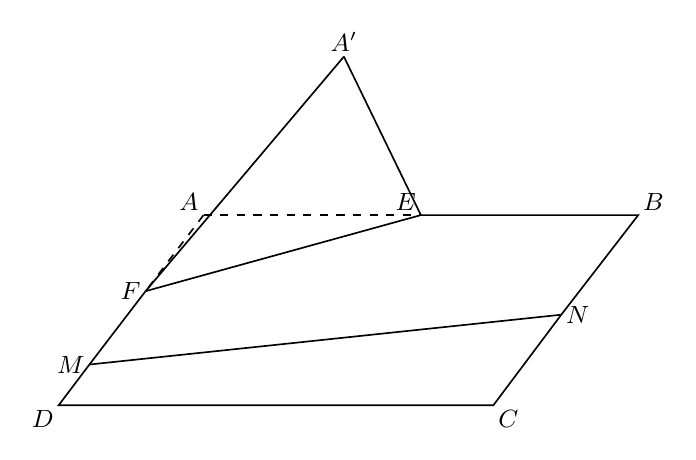
\begin{tikzpicture}[scale=1.15, semithick, every node/.style={inner sep=1.5pt, font=\small}]
  \coordinate (D) at (0,0);
  \coordinate (C) at (4.8,0);
  \coordinate (B) at (6.4,2.1);
  \coordinate (A) at (1.6,2.1);
  \coordinate (E) at (4.0,2.1);
  \coordinate (F) at (0.96,1.26);
  \coordinate (M) at (0.34,0.45);
  \coordinate (N) at (5.55,1.0);
  \coordinate (A1) at (3.15,3.85);

  % 矩形实线部分
  \draw (E) -- (B) -- (N) -- (C) -- (D) -- (M) -- (F);
  % 折痕 EF
  \draw (E) -- (F);
  % 翻折后的三角形
  \draw (A1) -- (E);
  \draw (A1) -- (F);
  % 原位置 A 的虚线
  \draw[dashed] (A) -- (E);
  \draw[dashed] (A) -- (F);
  % 第二折痕
  \draw (M) -- (N);

  \node[above] at (A1) {$A'$};
  \node[above left] at (A) {$A$};
  \node[above left] at (E) {$E$};
  \node[above right] at (B) {$B$};
  \node[left] at (F) {$F$};
  \node[left] at (M) {$M$};
  \node[right] at (N) {$N$};
  \node[below left] at (D) {$D$};
  \node[below right] at (C) {$C$};
\end{tikzpicture}
\end{center}
\nopagebreak[4]
\Needspace{0.4\textheight}
\end{question}
\endgroup
\begingroup
\renewenvironment{question}{\Needspace{0.5\textheight}}{}
\begin{question}
\gkti{21}已知 $m>1$，直线 $l:x-my-\dfrac{m^2}{2}=0$，椭圆 $C:\dfrac{x^2}{m^2}+y^2=1$，$F_1$，$F_2$ 分别为椭圆 $C$ 的左、右焦点。

（1）当直线 $l$ 过右焦点 $F_2$ 时，求直线 $l$ 的方程；

（2）设直线 $l$ 与椭圆 $C$ 交于 $A$，$B$ 两点，$\triangle AF_1F_2$，$\triangle BF_1F_2$ 的重心分别为 $G$，$H$。若原点 $O$ 在以线段 $GH$ 为直径的圆内，求实数 $m$ 的取值范围。
\nopagebreak[4]
\begin{center}% 2010 年浙江卷理科第 21 题：椭圆 C 与直线 l 交于 A、B 两点。
% 来源 PDF：普通高考/2010/2010浙江理.pdf，SHA-256 c61b26c8cab009d567644272afc34d81e3174ffa90244c333ecfb27d61034a00。
% 原页：第 2 页（A3 三栏）第 2 栏下部，书页码 640。
% 重绘依据：椭圆中心 O，x 轴向右、y 轴向上；直线 l 与椭圆交于右上 A、左下 B，
%   直线略偏离中心、不经过 O，照原页示意。
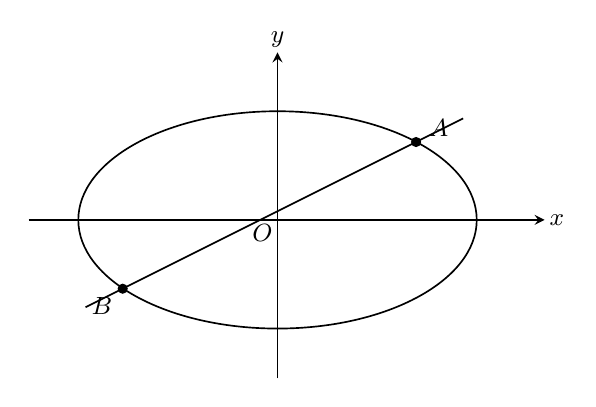
\begin{tikzpicture}[scale=1.15, semithick, every node/.style={inner sep=1.5pt, font=\small}]
  \draw (0,0) ellipse [x radius=2.2, y radius=1.2];

  % 坐标轴
  \draw[->, >=stealth] (-2.75,0) -- (2.95,0);
  \draw[->, >=stealth] (0,-1.75) -- (0,1.85);
  \node[right] at (2.95,0) {$x$};
  \node[above] at (0,1.85) {$y$};
  \node[below left] at (0,0) {$O$};

  % 直线 l 与交点
  \draw (-2.12,-0.965) -- (2.05,1.12);
  \fill (1.53,0.86) circle (1.6pt);
  \fill (-1.71,-0.76) circle (1.6pt);
  \node at (1.78,1.02) {$A$};
  \node at (-1.94,-0.95) {$B$};
\end{tikzpicture}
\end{center}
\nopagebreak[4]
\end{question}
\endgroup
\begin{question}
\gkti{22}已知 $a$ 是给定的实常数，设函数 $f(x)=(x-a)^2(x+b)\mathrm e^x$，$b\in\mathbf R$，$x=a$ 是 $f(x)$ 的一个极大值点。

（1）求 $b$ 的取值范围；

（2）设 $x_1$，$x_2$，$x_3$ 是 $f(x)$ 的 $3$ 个极值点，问是否存在实数 $b$，可找到 $x_4\in\mathbf R$，使得 $x_1$，$x_2$，$x_3$，$x_4$ 的某种排列 $x_{i_1}$，$x_{i_2}$，$x_{i_3}$，$x_{i_4}$（其中 $\{i_1,i_2,i_3,i_4\}=\{1,2,3,4\}$）依次成等差数列？若存在，求所有的 $b$ 及相应的 $x_4$；若不存在，说明理由。

\end{question}